% 中文对照校对稿 —— 与 main.tex（TVC 投稿版）逐节对应。
% 用途：中文校对，不用于投稿。编译：xelatex main_cn.tex
% 与 PRL 版的差异仅三处：(i) 补充材料并入正文；(ii) 新增 4.2 节“并行状态与单一状态”；
% (iii) 5.2 节明确写出“状态而非读出才是压缩瓶颈”。
\documentclass[UTF8,a4paper,11pt,fontset=windows]{ctexart}
\usepackage[margin=2.6cm]{geometry}
\usepackage{amsmath,amssymb,amsthm,bm,booktabs,graphicx,url,makecell}
\usepackage[hidelinks]{hyperref}
\graphicspath{{../figures/}}
\setlength{\emergencystretch}{1em}
\newtheorem{proposition}{命题}
\newtheorem{corollary}{推论}
\newcommand{\R}{\mathbb{R}}
\newcommand{\Sstate}{\mathbf{S}}
\newcommand{\vect}{\operatorname{vec}}

\title{面向流式点云识别的固定状态可加 FWP 网络}
\author{Dian Yu\\
University of New South Wales, Sydney, NSW 2052, Australia\\
\texttt{dian.yu2@student.unsw.edu.au}\\
ORCID：\url{https://orcid.org/0009-0002-0107-1014}}
\date{中文对照校对稿（对应 The Visual Computer 投稿版 main.tex）}

\begin{document}
\maketitle

\begin{abstract}
多数点云网络通过重新访问已保存的点、重建邻域或执行全局最大池化来获得上下文。这些操作适合离线处理，却使持续增长的点流依赖完整历史。PointProgrammerNet 用三个固定的 $128\times170$ 矩阵取代点历史。每个观测点产生一个表示“写到哪里”的归一化空间地址，以及一个表示“写入什么”的值向量；二者的外积直接加到矩阵中。这一简单构造使独立编码的分块可以通过矩阵加法精确合并，同时也支持相减和指数衰减。分割任务在指定坐标读取矩阵，分类任务则在删除全部输入点后仅使用矩阵。本文证明输入顺序不变性、分块与分布式编码等价性、固定保留内存，以及输出对新增证据的连续依赖。使用 XYZ 输入时，模型在 ShapeNetPart 上取得 $92.95\%$ 点准确率、$82.58\%$ 实例 mIoU 和 $79.10\%$ 类别 mIoU，在 ModelNet40 上取得 $86.59\%$ 分类准确率。三个 float32 状态始终占用 255 KiB，与点流长度无关。当累计点数达到 8,192 时，只更新新分块比重建完整状态快 $6.06\times$，相对状态误差仍低于 $10^{-6}$。这些结果展示了用有界、可直接更新与合并的状态取代不断增长的点历史时，所付出的精度代价与获得的实际收益。
\end{abstract}

\noindent\textbf{关键词：}点云；流式学习；可加状态；快速权重编程器；分割；分类

\section{引言}
点云是一个无序集合，但传感器是随时间观测它的。帧内处理应当与点的顺序无关，跨帧处理则不应要求重放完整历史。PointNet~\cite{qi2017pointnet} 通过对称最大池化获得全局描述子，PointNet++~\cite{qi2017pointnetplusplus} 构建多尺度度量邻域。两者在离线场景下都很有效。然而最大值不是一个可加状态：固定摘要通常无法通过简单相加来支持删除、独立分块合并以及带连续权重的证据累积。

本文研究一个更严格的设定：一个点在写入之后可以立即被丢弃。后续计算只访问固定矩阵，分割任务额外接收一个查询坐标。一个学习到的键把每个点分配到各个状态行上，一个二阶值记录质量、位置、学习内容与交叉矩。把这些逐点写入相加，就得到固定尺寸的状态。

因此，独立分块可以被合并，已保存的子集可以被减去，旧证据可以被衰减。新点更新状态时不需要再遍历此前的观测。同样的代数支持分布式感知：边缘设备编码不相交的区域或时间窗，传输固定矩阵，中心节点在分类或分割之前把这些矩阵相加。分割读取一个由坐标条件化的场，不保存任何历史点特征；分类只读取状态行，并丢弃完整点表。

本文的贡献是：
\begin{itemize}
\item 一个三尺度二阶快速权重编程器（FWP）状态，其内存不随观测点数增长；
\item 可加的逐点写入，支持精确的流式处理、层次化合并与分布式聚合，且无需重放分块内容；
\item 一个坐标条件化的分割读出头与一个仅依赖状态的分类读出头，两者都不对解码后的点做池化；
\item 覆盖可加性、状态运算、精度与更新代价的证明与实验，其中包含一个因果实验，表明在参数量相同的前提下三个并行状态优于单一状态。
\end{itemize}
本文的紧凑 PointNet++ 实现是受控基线，而非对原始工作的权威复现。我们用它们来度量固定状态这一约束所付出的精度代价。

\section{相关工作}
把无序点集压缩为固定摘要，已有若干成熟做法。它们的主要差别在于：在一个点被吸收的那一刻，各自放弃了什么。这个取舍决定了此后还有哪些状态运算可用。我们按这一取舍对相关工作分组，然后说明本架构保留了哪些性质。

\subsection{对称池化与度量邻域}
PointNet 先做逐点变换再做最大池化~\cite{qi2017pointnet}，PointNet++ 在此基础上加入层次化度量邻域~\cite{qi2017pointnetplusplus}，Deep Sets 刻画了由求和构建的置换不变函数~\cite{zaheer2017deepsets}。三者都与点序无关，且 Deep Sets 使用的求和在式~\eqref{eq:add-cn} 的严格意义下是可加的。但仍有两点限制了不断增长的点流。逐通道最大值丢弃了撤销它所需的信息，因此当某个观测之后被移除时，已保存的摘要无法被修正。度量邻域是相对于当前持有的点定义的，因此插入或删除一个点会改变其他点属于哪些邻域，分组必须重建。Deep Sets 避开了这两点，但它求和进一个单一的全局向量，该向量不携带空间地址，因而无法在某个被请求的坐标上求值。PointProgrammerNet 保留了可加的求和，并把它铺展到 128 个带空间地址的行上；正是这一点使坐标条件化的读取成为可能，同时不放弃可加性。

\subsection{基于学习中心的固定尺寸摘要}
VLAD 把局部描述子分配到学习到的中心并累加残差，从而压缩表示~\cite{jegou2010vlad}。NetVLAD 把该分配变为软分配且可微~\cite{arandjelovic2016netvlad}，PointNetVLAD 把这一构造用于点云的地点识别~\cite{uy2018pointnetvlad}。其累加器与我们的形状相同：一个由软分配到学习中心而构建的固定矩阵。三点差别是重要的。其一，被累加的残差是一阶的，而式~\eqref{eq:value-cn} 保留了直到二阶的全部矩。其二，分配是在特征空间中进行的，而我们的地址是坐标的归一化函数，因而对查询位置保持连续。其三，也是与本文最相关的一点：NetVLAD 先对每个块做块内归一化，再对展平后的描述子做 $L_2$ 归一化。这些步骤不是可加的——把两个部分描述子各自归一化后再相加，并不能复现二者并集的描述子。原始累加器本身是可加的，但已发表的构造把这一性质归一化掉了，且从未使用它。我们刻意让累加器保持未归一化，并把归一化推迟到读出时刻，这正是命题~\ref{prop:order-cn} 得以成立的原因。

\subsection{对固定隐变量集合的注意力}
Set Transformer 使用诱导点与注意力对集合作摘要~\cite{lee2019settransformer}。Perceiver IO 维护一个尺寸与输入无关的隐变量数组，并通过一组输出查询对该隐变量做注意力，从而解码任意输出，包括逐元素的稠密预测~\cite{jaegle2022perceiverio}。「用查询读取固定隐变量以产生稠密输出」这一想法属于他们，而不属于本文。差别在编码端。softmax 交叉注意力在观测元素上做归一化，因此由两个不相交分块得到的隐变量并不等于两个隐变量之和；该表示无法通过算术进行合并、相减或衰减，原文也未主张任何此类性质。我们的写入不在观测集合上施加任何归一化，因此状态始终是一组彼此独立的逐点项之和。查询的含义也不同：Perceiver 的查询是学习到的位置嵌入，而我们的查询是与数据处于同一空间中的坐标，因此同一个状态可以在从未被观测过的位置上求值。

\subsection{有界的循环状态}
核化注意力可以用固定尺寸状态以循环方式求值~\cite{katharopoulos2020transformers}，快速权重编程器把这类更新表达为可加外积或 delta 修正~\cite{schlag2021linear}。这些正是我们的写入所使用的机制。近期点云工作也通过结构化状态空间模型采用有界状态；PointMamba 在循环之前用空间填充曲线把点序列化~\cite{liang2024pointmamba}。序列化使隐状态成为遍历顺序的函数，因此它不是置换不变的，两个部分状态也无法相加。我们保留有界状态，但不保留序列，因为正是与顺序无关的求和换来了分块与设备等价性。

\subsection{本架构拒绝做的事}
上述每一族都为换取某项性质而交出了另一项。最大值交出了可逆性。度量邻域交出了编辑的局部性。归一化描述子交出了可加性。softmax 编码器交出了可分解性。序列化的循环交出了顺序不变性。本文的设计源自写入时刻的一条拒绝：任何把某个点的写入与另一个点耦合起来的东西，都不得进入持久状态。这排除了在观测集合上的归一化、点与点之间的比较、选择与排序。聚合方法通常在吸收一个点时所做的运算——密度归一化、相对参考位置的中心化，以及非线性解释——在这里都被推迟到读出，从而不再触及所存矩阵的代数。表~\ref{tab:family-comparison-cn} 给出由此确定的位置。

\begin{table}[t]
\centering
\caption{各族集合摘要所保留的性质。「顺序无关写入」指摘要不依赖点被吸收的顺序；「可加状态」指并集的摘要等于各摘要之和；「有界状态」指保留内存不随观测点数增长；「坐标读取」指仅凭摘要即可在被请求的位置上求值。}
\label{tab:family-comparison-cn}
\small
\begin{tabular}{lcccc}
\toprule
族 & \makecell{顺序无关\\写入} & \makecell{可加\\状态} & \makecell{有界\\状态} & \makecell{坐标\\读取} \\
\midrule
PointNet，最大池化 & 是 & 否 & 是 & 否 \\
PointNet++，度量邻域 & 是 & 否 & 否 & 否 \\
Deep Sets，全局求和 & 是 & 是 & 是 & 否 \\
VLAD、NetVLAD、PointNetVLAD & 是 & 否$^{a}$ & 是 & 否 \\
Set Transformer、Perceiver IO & 是 & 否$^{b}$ & 是 & 是$^{c}$ \\
线性注意力、快速权重 & 序列 & 是 & 是 & 否 \\
序列化点上的状态空间模型 & 否 & 否 & 是 & 否 \\
\midrule
PointProgrammerNet（本文） & 是 & 是 & 是 & 是 \\
\bottomrule
\end{tabular}
\\[3pt]
\parbox{\linewidth}{\footnotesize $^{a}$原始累加器是可加的，但块内归一化与 $L_2$ 归一化移除了该性质。$^{b}$在观测元素上的 softmax 把它们耦合在一起。$^{c}$Perceiver IO 从学习到的位置查询解码稠密输出，而非从输入空间中的坐标。}
\end{table}

这一拒绝的代价是被测量出来的，而不是被断言的。表~\ref{tab:segmentation_accuracy_cn} 与表~\ref{tab:classification_accuracy_cn} 报告了与层次化基线的精度差距，第~\ref{sec:parallel-cn} 节则表明，挽回其中一部分的是并行状态结构，而不是参数预算。

我们在 ModelNet40~\cite{wu20153dshapenets} 上评估分类，在 ShapeNetPart~\cite{yi2016scalable} 上评估部件分割，后者派生自 ShapeNet~\cite{chang2015shapenet}。

\section{方法}
设 $X=\{\bm{x}_i\}_{i=1}^N$，归一化坐标 $\bm{x}_i\in\R^3$。PointProgrammerNet 用三个矩阵 $\Sstate_s\in\R^{128\times170}$ 取代不断增长的点历史，其中 $s\in\{f,m,b\}$ 表示初始半径分别为 $0.08$、$0.20$ 和 $0.60$ 的三个分支。半径、空间中心、点编码器与读出网络都独立学习。状态是为每个物体或点流创建的，与训练得到的模型参数相互独立。

三个分支的状态尺寸相同，使用相同的方程。不同的初始半径只提供不同的起始条件；每个分支最终表示什么由训练决定。分支首先用一个两层点网络把坐标映射为学习内容，
\begin{equation}
\bm g_s(\bm x)=\operatorname{ReLU}\!\left(\operatorname{BN}\!\left(W_{s2}
\operatorname{ReLU}(\operatorname{BN}(W_{s1}\bm x+\bm b_{s1}))+\bm b_{s2}\right)\right)
\in\R^{32}.
\label{eq:content-cn}
\end{equation}
矩阵 $W_{s1},W_{s2}$ 与偏置在每个分支中独立学习，两个隐藏层宽度均为 32。因此状态尺寸相同并不意味着特征重复。该非线性映射对每个点独立求值，所以它丰富了一个点所写入的内容，却没有把这次写入与任何其他点耦合；可加性得以保持，是因为持久状态中累加的只有随后的外积。

\begin{figure}[t]
\centering
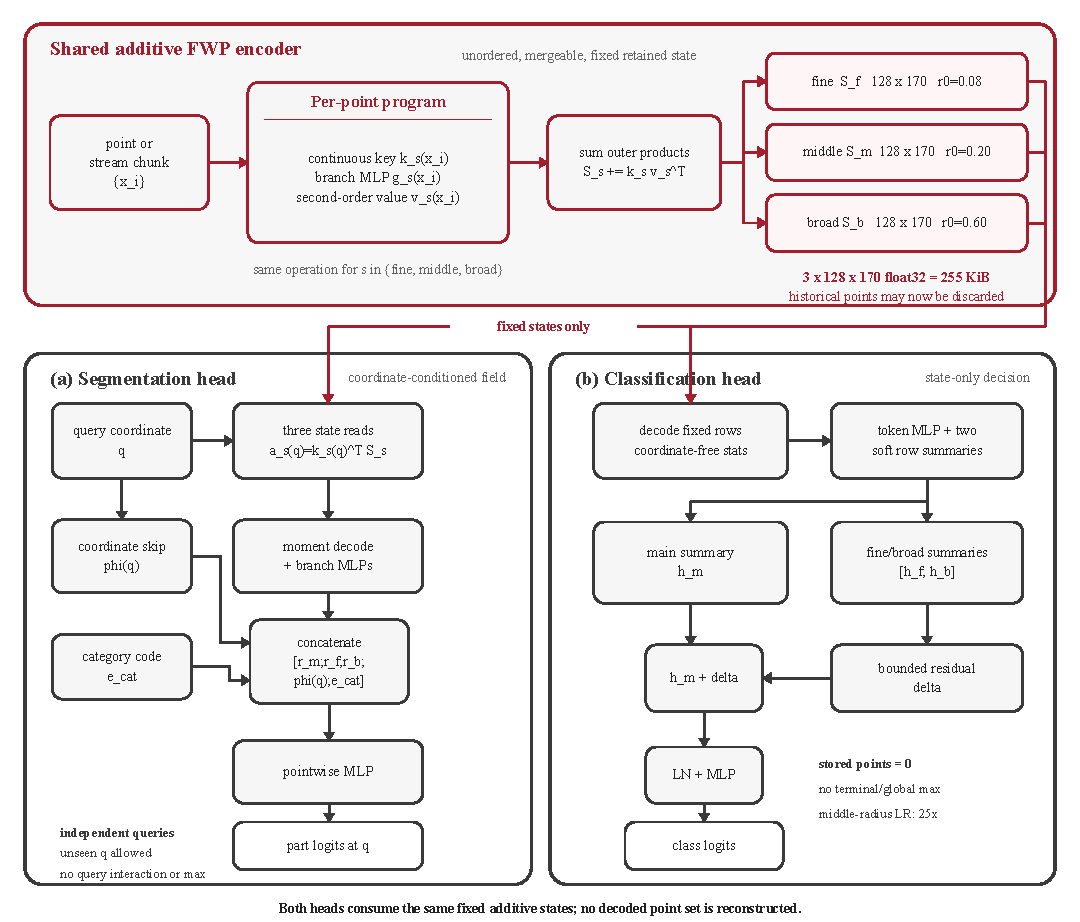
\includegraphics[width=\linewidth]{fig00_pointprogrammernet_architecture.pdf}
\caption{PointProgrammerNet 架构。红色路径承载三个等尺寸可加 FWP 状态，此时历史点已被丢弃。分割头在查询坐标 $\bm q$ 处读取每个状态，然后拼接解码得到的上下文、坐标跳连与类别编码。分类头解码固定行，并把一个有界的“细—粗”残差加到中尺度摘要上。两个读出头都不重建也不池化任何解码点集。}
\end{figure}

\subsection{可加状态的构造}
128 个状态行各有一个学习到的中心 $\bm c_{sj}\in\R^3$。这些中心不是从输入点云中采样的。训练之前，用一个 Sobol 序列在 $[-0.9,0.9]^3$ 内放置 128 个初始锚点，使各行一开始就有较宽的空间覆盖。每个分支拥有自己可训练的一份副本，训练过程可以通过有界参数化 $\bm c_{sj}=0.95\tanh(\bm\theta_{sj})$ 移动这些锚点。对一个观测坐标 $\bm x$，分支计算它到全部 128 个锚点的距离，并把这些距离转换为 128 个连续的写入份额。正半径 $r_s=\exp(-\lambda_s)$ 控制这些份额的集中程度。归一化地址为
\begin{equation}
k_{sj}(\bm x)=\frac{\exp[-\|\bm x-\bm c_{sj}\|^2/(2r_s^2)]}
{\sum_{u=1}^{128}\exp[-\|\bm x-\bm c_{su}\|^2/(2r_s^2)]}.
\label{eq:key-cn}
\end{equation}
分母把每个点的总写入质量固定为 1。这避免了稠密分块改变单次写入的尺度，也使半径只控制集中度而不控制总量。直观地说，这些中心相当于 128 个软空间箱。靠近若干中心的点会给这些行较大份额、给其余行很小份额；它绝不会只被分配给一个箱。地址决定点写到哪里，而下面这个 170 维的值决定它贡献哪些统计量：
\begin{equation}
\bm v_s(\bm x)=[1,\bm x,\bm g_s,\vect(\bm x\bm g_s^\top),
 x^2,y^2,z^2,xy,xz,yz,\bm g_s\odot\bm g_s].
\label{eq:value-cn}
\end{equation}
各块维度为 $1+3+32+96+6+32=170$，分别保留质量、一阶矩、学习内容、坐标—内容乘积与二阶矩。开头的 1 之后用作局部平均的分母。六个坐标二次项与 32 个特征平方项保留了均值无法恢复的离散程度。等价地说，值向量收集了 $(\bm x,\bm g_s)$ 直到二阶的全部矩，只是把特征—特征块限制在其对角线上，使其宽度对内容维度保持线性。

\begin{table}[t]
\centering
\caption{单个点写入的值。每个状态行都有这 170 列。}
\label{tab:value-layout-cn}
\begin{tabular}{lrl}
\toprule
块 & 维度 & 保留的信息 \\
\midrule
$1$ & 1 & 累计质量 \\
$\bm x$ & 3 & 坐标和 \\
$\bm g_s$ & 32 & 学习内容和 \\
$\bm x\bm g_s^\top$ & 96 & 位置—内容关系 \\
$\bm x\bm x^\top$ & 6 & 几何二阶矩 \\
$\bm g_s\odot\bm g_s$ & 32 & 特征二阶矩 \\
\bottomrule
\end{tabular}
\end{table}

一个点对状态行 $j$ 的改变为
\begin{equation}
[\Delta\Sstate_s(\bm x)]_{j,:}=k_{sj}(\bm x)\bm v_s(\bm x)^\top .
\label{eq:single-write-cn}
\end{equation}
这一秩一更新使用的正是 FWP 的定义性操作：键选择写到哪里，值提供写入什么，独立的写入通过相加叠加~\cite{schlag2021linear}。PointProgrammerNet 保持了这种线性叠加，既没有在观测点集上做写入归一化，也没有对先前状态做非线性覆写。因此一行是一个加权累加器，而不是某个被选中点的槽位；把这些外积相加得到
\begin{equation}
\Sstate_s(X)=\sum_{i=1}^{N}\bm k_s(\bm x_i)\bm v_s(\bm x_i)^\top
=\bm K_s^\top\bm V_s.
\label{eq:state-cn}
\end{equation}
没有点被分配给单一行，也没有点与另一个点作比较。一旦它的三个外积被加入，它就可以被释放。

对新到达的分块，$\bm K_s\in\R^{M\times128}$ 堆叠其地址，$\bm V_s\in\R^{M\times170}$ 堆叠其值。分块更新就是一次矩阵乘积 $\Delta\Sstate_s=\bm K_s^\top\bm V_s$。持久状态按 $\Sstate_s\leftarrow\Sstate_s+\Delta\Sstate_s$ 更新，此后 $\bm K_s$、$\bm V_s$ 以及分块中的点都可以丢弃。分块大小只改变临时工作内存，不改变保留下来的表示。

因此完整的流式流程很短。对每个到达的分块，编码器（i）在共享参考系中归一化其坐标，（ii）计算三组地址与值矩阵，（iii）把三个乘积 $\bm K_s^\top\bm V_s$ 加到持久状态上，（iv）释放全部与分块相关的张量。独立设备执行同样的四步，并只传输它们的三个矩阵。推理时，分割头只在被请求的坐标上求值，分类头则直接消费这些矩阵。后续任何阶段都不需要从状态重新生成点表。

\subsection{任务读出}
在分割中，$\bm x_i$ 表示一个已经被加入状态、随后可被丢弃的观测点；$\bm q$ 仅仅是请求标签的那个坐标。在 ShapeNetPart 上，查询使用带标注的输入坐标，但解码器接收的是坐标与固定状态，而不是保存下来的点特征。查询通过式~\eqref{eq:key-cn} 产生地址并读取
\begin{equation}
\bm a_s(\bm q)=\bm k_s(\bm q)^\top\Sstate_s
=\sum_i \underbrace{\bm k_s(\bm q)^\top\bm k_s(\bm x_i)}_{w_{si}(\bm q)}
\bm v_s(\bm x_i)^\top .
\label{eq:effective-read-cn}
\end{equation}
系数 $w_{si}(\bm q)$ 是对该矩阵读取的代数解释：当点 $i$ 强烈写入了 $\bm q$ 强烈读取的那些行时，它就大。实现直接计算左端的矩阵乘积；它既不重建也不重访点 $i$，也不对解码点做全局最大池化。

$\bm a_s(\bm q)$ 的第一个分量是读取质量 $\mu_s(\bm q)$。实现通过下式避免在近乎空白区域出现不稳定的除法：
\begin{equation}
\epsilon_s=10^{-3}\operatorname{mean}_{\bm q'}\mu_s(\bm q')+10^{-20},
\qquad
\widetilde\mu_s(\bm q)=\max(\mu_s(\bm q),\epsilon_s).
\label{eq:seg-floor-cn}
\end{equation}
其中的均值在单个样本的查询坐标上取，并从梯度中分离。式~\eqref{eq:seg-floor-cn} 中的 $\max$ 只是一个标量数值下限；它既不比较点特征，也不执行全局最大池化。把保存的坐标、特征、交叉乘积与平方和除以 $\widetilde\mu_s$，得到局部坐标均值与特征均值 $\bar{\bm x}_s,\bar{\bm g}_s$、交叉矩 $E_{xg,s}$、几何矩 $E_{xx,s}$ 与特征能量 $E_{gg,s}$。它们构成 170 维描述子
\begin{equation}
\begin{aligned}
\bm d_s(\bm q)=[&\bar{\bm g}_s,\bar{\bm x}_s-\bm q,\log\widetilde\mu_s,
\vect(E_{xg,s}-\bm q\bar{\bm g}_s^\top),\\
&\operatorname{vech}(E_{xx,s}-\bar{\bm x}_s\bar{\bm x}_s^\top),
\sqrt{[E_{gg,s}-\bar{\bm g}_s\odot\bar{\bm g}_s]_++10^{-8}}].
\end{aligned}
\label{eq:query-descriptor-cn}
\end{equation}
其中 $\operatorname{vech}$ 保留对称 $3\times3$ 矩阵的六个不同元素，$[\cdot]_+$ 截去由舍入误差造成的负方差。其块维度为 $32,3,1,96,6,32$，同样合计 170。该描述子刻意组合了互补的统计量：特征均值提供局部语义内容，相对质心与几何协方差描述局部位置与形状，对数质量记录有多少证据支撑这次读取；坐标—特征项保留了内容在查询点周围如何变化，特征标准差则暴露出仅凭均值会被掩盖的混合与边界变化。每个分支使用同一个 $170\rightarrow160\rightarrow160$ 的 BatchNorm--ReLU 解码器。最终的逐点头为
\begin{equation}
\bm z_{\rm seg}(\bm q)=h_{\rm seg}([\bm r_f(\bm q);\bm r_m(\bm q);
\bm r_b(\bm q);\phi(\bm q);\bm e_{\rm cat}]),
\label{eq:seg-cn}
\end{equation}
其中 $\bm r_s\in\R^{160}$ 是一次解码后的状态读取，$\phi(\bm q)\in\R^{32}$ 是坐标特征，$\bm e_{\rm cat}\in\R^{16}$ 是 ShapeNetPart 的类别编码。分割 MLP 为 $528\rightarrow256\rightarrow128\rightarrow50$，前两个仿射层之后带 BatchNorm、ReLU 与 dropout $0.3$。坐标通路是绕过状态压缩的类 U-Net 跳连。该头对每个查询单独作用，从不在解码点之间做池化。历史特征可以删除，只有之后要被标注的坐标必须保留。同一个固定状态也可以在未被观测过的坐标上查询。

在分类中不保留任何坐标。对第 $j$ 行，保存的 170 个元素按下式划分：
\[
[\mu_{sj},\bm p_{sj},\bm f_{sj},\vect(\bm C_{sj}),
\operatorname{vech}(\bm Q_{sj}),\bm u_{sj}],
\]
即质量、坐标和、特征和、坐标—特征和、对称坐标二阶矩与特征平方和。行归一化使用
\begin{equation}
\widetilde\mu_{sj}=\max\!\left(
\mu_{sj},10^{-4}R^{-1}\sum_{u=1}^{R}|\mu_{su}|+10^{-20}\right),
\label{eq:cls-floor-cn}
\end{equation}
其下界在反向传播中被分离。记 $\bar\mu_s=R^{-1}\sum_u\widetilde\mu_{su}$，除以 $\widetilde\mu_{sj}$ 得到
\begin{equation}
\begin{aligned}
\bm d^{\rm row}_{sj}=[&
\bar{\bm g}_{sj},\bar{\bm x}_{sj},
\log(\widetilde\mu_{sj}/\bar\mu_s),
\operatorname{vech}(\operatorname{Cov}_{xx,sj}),\\
&\operatorname{Std}_{g,sj},
\vect(\operatorname{Cov}_{xg,sj})]\in\R^{170},
\end{aligned}
\label{eq:cls-descriptor-cn}
\end{equation}
块维度为 $32,3,1,6,32,96$。一个独立的 $170\rightarrow128\rightarrow128$ LayerNorm--GELU 网络编码每一行，得到 $\bm T_s\in\R^{128\times128}$。两列学习到的打分对固定行做摘要：
\begin{equation}
\bm U_s=\operatorname{softmax}_{\rm rows}(\operatorname{score}_s(\bm T_s)),\qquad
\bm h_s=H_s(\vect(\bm U_s^\top\bm T_s))\in\R^{256}.
\label{eq:state-summary-cn}
\end{equation}
这个 softmax 作用在 128 个保留的状态行上，而不是作用在输入点上，因此编码之后其代价是固定的。中尺度摘要作为参考，另外两个构成有界残差：
\begin{align}
\bm\delta&=\sigma(a)\tanh(W[\bm h_f;\bm h_b]+\bm b),\nonumber\\
\bm z_{\rm cls}&=h_{\rm cls}(\operatorname{LN}(\bm h_m+\bm\delta)).
\label{eq:cls-cn}
\end{align}
残差投影从零开始，$\sigma(a)$ 从 $0.1$ 开始。分类器 $h_{\rm cls}$ 为 $256\rightarrow256\rightarrow40$，带 GELU 与 dropout $0.3$。所有半径都可学习；只有中尺度半径使用 $25\times$ 学习率倍数与零权重衰减。分类器只使用固定矩阵，末端没有任何点最大池化。两列打分为每个状态提供互补的、代价固定的视角，而不是把所有行都压成一个平均。以中尺度分支作为初始稳定的参考、并让细尺度与粗尺度摘要经由一个零起点的有界残差进入，可以避免三个分支在各自学到有用摘要之前互相干扰；当辅助证据确实有助于分类时，该残差随后可以增大。

\subsection{流式性质}
对任意点多重集 $A$ 与 $B$，式~\eqref{eq:state-cn} 给出
\begin{equation}
\Sstate_s(A\uplus B)=\Sstate_s(A)+\Sstate_s(B).
\label{eq:add-cn}
\end{equation}
有限和同时也使状态与点的顺序无关。因此，分别编码的分块、设备或聚合树的分枝都可以通过相加合并。若可移除子集的状态可用，就可以将其减去；指数遗忘使用 $\Sstate_{s,t}=\rho\Sstate_{s,t-1}+\Sstate_s(X_t)$。精确的分布式等价性要求共同的训练权重、坐标归一化与参考系。

记 $F_s(\bm x)=\bm k_s(\bm x)\bm v_s(\bm x)^\top$ 为单个点的秩一 FWP 写入，于是 $\Sstate_s(X)=\sum_{\bm x\in X}F_s(\bm x)$。

\begin{proposition}[顺序、分块与设备]
\label{prop:order-cn}
对点多重集 $A,B$，有 $\Sstate_s(A\uplus B)=\Sstate_s(A)+\Sstate_s(B)$，且状态与点的顺序无关。使用相同训练编码器、坐标归一化与参考系的设备，因而可以通过把各自独立编码的状态相加而得到集中式状态。
\end{proposition}
\begin{proof}
两端展开为同一组有限的逐点矩阵 $F_s(\bm x)$。在实数运算下，重排或重新分组一个有限和不改变其值。float32 结果的差异仅来自累加顺序。
\end{proof}

为把分布式主张写清楚，设设备 $d$ 观测点多重集 $X^{(d)}$，且所有设备使用同一个编码器。中心节点构造
\begin{equation}
\Sstate_s^{\rm global}=\sum_{d=1}^{D}\Sstate_s(X^{(d)})
=\Sstate_s\!\left(\biguplus_{d=1}^{D}X^{(d)}\right).
\label{eq:distributed-cn}
\end{equation}
该等式由两端展开为同一组逐点外积之和得到。无论部分状态是同时到达、异步到达，还是经过一棵中间聚合树，它都成立。分类随后只使用合并后的矩阵。分割则额外接收待查询的坐标与物体类别编码。原始点特征无需离开感知设备。

同样的代数在所需部分状态可用时给出可逆的状态运算。若 $Y$ 是一个已知子集，则 $\Sstate_s(X\setminus Y)=\Sstate_s(X)-\Sstate_s(Y)$。这在不重放 $X$ 的情况下移除了 $Y$ 的聚合贡献。在追加之前乘以 $\rho\in[0,1]$ 即实现指数遗忘。这些陈述针对表示本身；当某子集的独立状态未被保留时，相减无法从状态中恢复其中的单个点。

\begin{proposition}[保留内存与更新代价]
\label{prop:memory-cn}
若每个分支有 $R_s$ 行、$D_s$ 列，则保留内存为 $O(\sum_sR_sD_s)$，与历史长度无关。编码 $M$ 个新点的代价为 $O(M\sum_sR_sD_s)$，且不重访更早的观测。
\end{proposition}
\begin{proof}
只有固定矩阵是持久的。无论此前有多少分块，一个新分块都只贡献同样维度的新外积。
\end{proof}

为刻画一个逐渐到达的观测，用证据强度 $t\in[0,1]$ 缩放其写入：
\begin{equation}
\Sstate_s(t)=\Sstate_s^{\rm old}+t\,\bm k_s(\bm x)\bm v_s(\bm x)^\top .
\label{eq:continuous-cn}
\end{equation}
状态对 $t$ 是仿射的。高斯地址、softmax、带正下限的归一化矩读取、仿射层、BatchNorm 或 LayerNorm、ReLU 或 GELU，以及稳定化的平方根都是连续的。它们的复合使分类 logits 与固定坐标下的分割 logits 对 $t$ 连续且分段光滑。空间地址对查询坐标 $\bm q$ 也是连续的，因此一个固定状态定义了一个连续、分段光滑的分割场。这并不意味着硬 argmax 标签会连续变化：当两个 logits 交叉时它仍可跳变。它也不能建立校准性或“证据越多必然越好”的单调性。

对已发布的配置，三个分支的 $R_s=128$、$D_s=170$，因此持久表示包含 65,280 个数。以 float32 计为每个点流 261,120 字节（255 KiB）。临时张量随到达分块的大小变化，可以立即释放。分割应用可以保留一小组感兴趣的坐标，但这些坐标是外部查询，而不是历史状态的一部分；分类应用则完全不保留坐标。

可加规则把所有帧视为可交换的证据。当帧的顺序本身应当改变记忆时，未来的扩展可以采用帧级的快速权重 delta 更新~\cite{schlag2021linear}：
\begin{equation}
\Sstate_{s,t}=\rho\Sstate_{s,t-1}+\eta_t\bm K_{s,t}^{\top}
(\bm V_{s,t}-\bm K_{s,t}\Sstate_{s,t-1}).
\label{eq:delta-cn}
\end{equation}
其中 $\bm K_{s,t}$ 与 $\bm V_{s,t}$ 打包第 $t$ 帧中的全部键与值，$\rho$ 保留旧状态，$\eta_t$ 是更新率。在帧内重排点相当于对两个矩阵同时左乘同一个置换 $P$；由于 $P^\top P=I$，修正项不变。因此该扩展保持帧内点序不变性，同时引入帧间有序的状态转移。它是一个提出的方向，未用于本文报告的实验，因为它有意放弃了跨帧的精确可加性。

\section{实验}
\subsection{协议与精度}
我们把每个物体居中，并将 XYZ 除以其最大绝对坐标，使用 1,024 个点。ShapeNetPart 含 13,972 个训练形状与 2,874 个测试形状；ModelNet40 含 9,840 与 2,468 个。模型用 AdamW 训练 20 个 epoch，基础学习率 $3\times10^{-3}$，权重衰减 $10^{-4}$，余弦衰减，批大小分别为 16 与 32。分类使用 0.1 的标签平滑。结果为种子 0、1、2 上的均值 $\pm$ 总体标准差。分割模型含 341,909 个可训练参数，纯状态分类器含 529,426 个。在分类中，只有中尺度半径使用 $25\times$ 学习率倍数且不加权重衰减；第~\ref{sec:screens-cn} 节的受控筛选说明了这一面向鲁棒性的选择。所报告的全部 PointProgrammerNet 变体都使用三个 $128\times170$ 状态，且在输入点或解码点上都没有全局最大池化。我们的紧凑 PointNet++ 实现是本地受控基线，而非权威复现。

\begin{table}[t]
\centering
\caption{ShapeNetPart 分割（XYZ 输入）。PointProgrammerNet 从不在解码查询点上做池化。}
\label{tab:segmentation_accuracy_cn}
\begin{tabular}{lrrrr}
\toprule
模型 & 点准确率 (\%) & 实例 mIoU (\%) & 类别 mIoU (\%) & 参数量 \\
\midrule
轻量 PointNet++ & $93.41\pm0.05$ & $83.88\pm0.11$ & $79.51\pm0.24$ & 573,106 \\
PointProgrammerNet & $92.95\pm0.02$ & $82.58\pm0.15$ & $79.10\pm0.25$ & 341,909 \\
\bottomrule
\end{tabular}
\end{table}
PointProgrammerNet 的点准确率比轻量 PointNet++ 对照低 0.46 个百分点，实例 mIoU 低 1.30 个百分点，而参数量少 40.3\%。

\begin{table}[t]
\centering
\caption{ModelNet40 分类（1,024 点）。Density 指固定的密度梯度偏移。}
\label{tab:classification_accuracy_cn}
\begin{tabular}{lrrrr}
\toprule
模型 & 干净 (\%) & 密度 (\%) & 掉分 (pp) & 参数量 \\
\midrule
轻量 PointNet++ & $89.84\pm0.43$ & $85.47\pm0.88$ & $4.38\pm1.18$ & 207,784 \\
参数对齐的 PointNet & $87.90\pm0.27$ & $87.55\pm0.38$ & $0.35\pm0.12$ & 442,838 \\
PointProgrammerNet & $86.59\pm0.23$ & $82.47\pm0.93$ & $4.12\pm0.71$ & 529,426 \\
\bottomrule
\end{tabular}
\end{table}
纯状态分类器达到 $86.59\%$ 的干净准确率，比轻量 PointNet++ 低 3.25 个百分点，比参数对齐的 PointNet 低 1.31 个百分点。其密度偏移准确率为 $82.47\%$。这量化了“丢弃点表、只从可合并状态分类”所付出的精度代价。

\subsection{并行状态与单一状态}
\label{sec:parallel-cn}
三个状态并非冗余，其收益也不是参数量效应。我们用一个严格配对的因果实验来验证：对照组保留完整模型及其初始化，但移除两路辅助读取，使得只有主状态能够影响输出。因此两侧的参数量与初始权重完全相同。表~\ref{tab:parallel_states_cn} 报告了该筛选实验，训练 5 个 epoch，种子 0、1、2，使用 2,048 个训练形状与 512 个测试形状。

\begin{table}[t]
\centering
\caption{并行状态与单一状态的对比。5 个 epoch 的筛选实验，三个种子，2,048 训练形状与 512 测试形状。单状态对照保留完整模型与初始化，但移除两路辅助读取。}
\label{tab:parallel_states_cn}
\begin{tabular}{lrrrr}
\toprule
配置 & 状态数 & 参数量 & 实例 mIoU (\%) & 类别 mIoU (\%) \\
\midrule
仅主状态（因果对照） & 1 & 484,914 & 74.68 & 70.50 \\
主状态加宽至 256 行 & 3 & 485,298 & 74.79 & 70.53 \\
并行状态，保守半径学习率 & 3 & 484,914 & 75.73 & 71.03 \\
并行状态，更强残差混合 & 3 & 484,914 & 75.88 & 70.97 \\
\midrule
已发布的三状态模型 & 3 & 341,909 & 77.22 & 73.08 \\
\bottomrule
\end{tabular}
\end{table}

在参数量不变的前提下，移除两个辅助状态使实例 mIoU 下降 $1.05$ 至 $1.20$ 个百分点。改为给某一个状态增加容量同样无济于事：在保留三个状态的前提下把主状态从 128 行加倍到 256 行，只达到 $74.79$，仍低于任何一个所有状态均为 128 行的配置。已发布模型使用三个状态、341,909 参数，在同一筛选协议下达到 $77.22$，比单状态对照高出 $2.54$ 个百分点，而参数量少 29.5\%。因此，并行状态所贡献的可用结构，既不是更大的参数预算能提供的，也不是加宽主状态能提供的。这些是在数据子集上的短程筛选，作为受控比较报告，而不作为最终精度。

\subsection{可加性与更新代价}
在 32 个物体上，由 2--32 个有序或打乱分块构建的状态与一次性构建的结果一致，相对误差低于 $5.3\times10^{-7}$。追加、合并、移除与衰减测试均低于 $9.8\times10^{-7}$。三个 float32 状态含 65,280 个标量（255 KiB），与点流长度无关。对短点云而言原始 XYZ 更小；其收益在于有界的保留内存，以及在长流或分布式场景中可直接进行的状态运算。

\begin{figure}[t]\centering
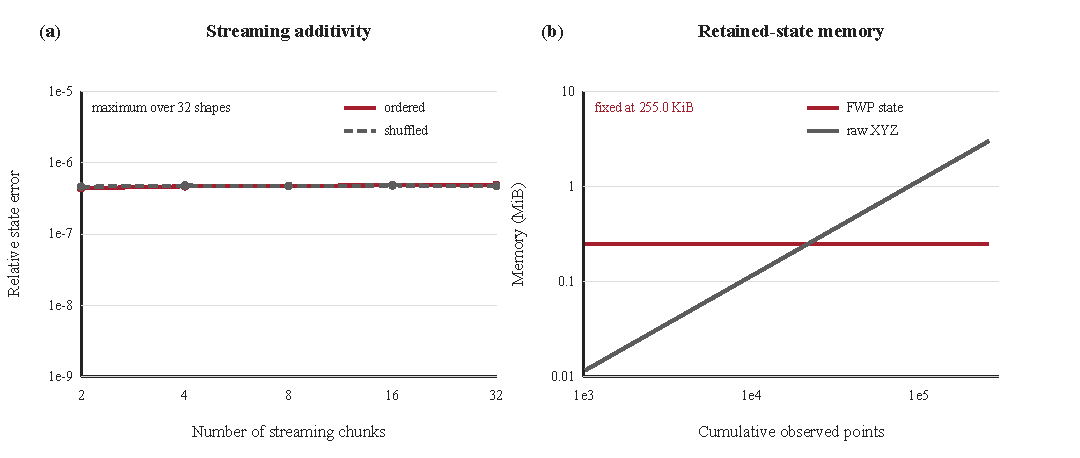
\includegraphics[width=0.92\linewidth]{fig01_additivity_fixed_state.pdf}
\caption{可加流式处理与固定保留内存。有序与打乱的分块写入都能复现单批次 FWP 状态，误差仅为浮点累加误差。三个 $128\times170$ 的 float32 状态始终占用 255 KiB，而保存 XYZ 坐标的开销随观测数线性增长。}
\end{figure}

\begin{figure}[t]\centering
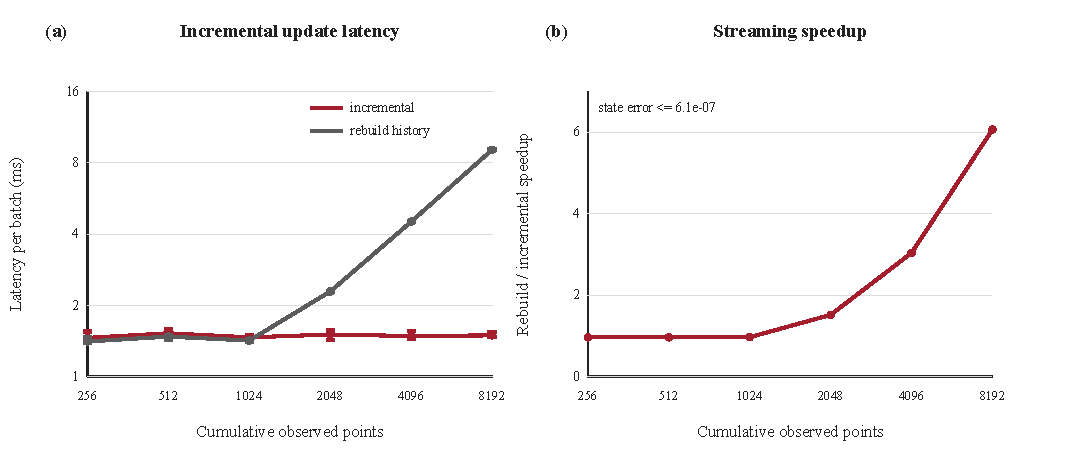
\includegraphics[width=0.92\linewidth]{fig04_streaming_efficiency.pdf}
\caption{设备端点流的 FWP 状态构建代价。（a）增量更新只处理一个新的 256 点帧，而重建要处理全部累计点。数值为四个点流、7 次交错试验、每次 30 遍重复的中位墙钟时延，误差棒表示观测范围。（b）加速比随历史长度增长，同时增量状态与重建状态在数值上保持等价。}
\end{figure}
在一块 RTX 3070 Ti Laptop GPU 上，四个点流每帧接收 256 个新点。增量时延稳定在 1.46--1.53 ms，而重建时延随历史增长。在累计 2,048、4,096 和 8,192 个点时，更新分别快 $1.52\times$、$3.04\times$ 和 $6.06\times$。在累计点数约 512 以下时，两条路径代价相当，重建甚至略快，因此该优势是渐近的而非普遍的。

\subsection{状态代数的实际验证}
\begin{figure}[t]\centering
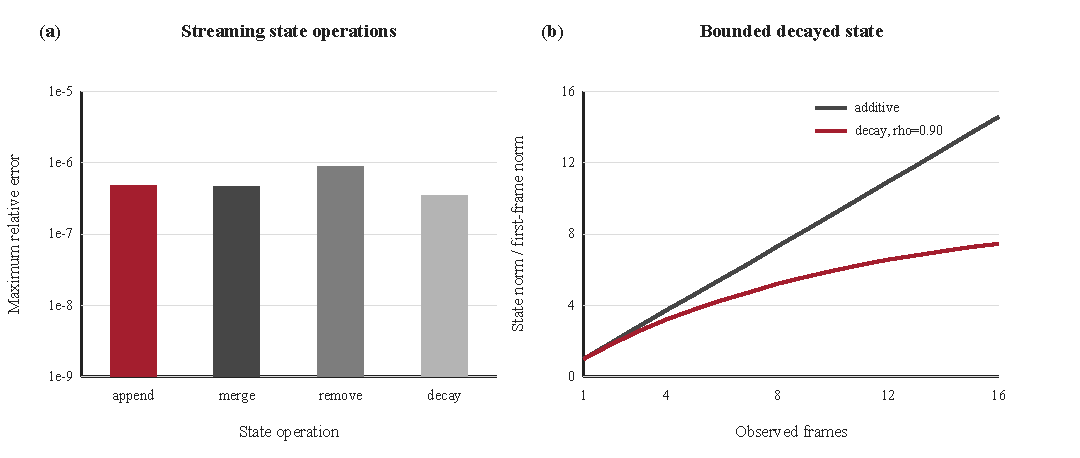
\includegraphics[width=0.92\linewidth]{fig02_state_operations.pdf}
\caption{流式状态运算。（a）在 32 个 ShapeNetPart 物体上，追加/合并、帧移除与指数衰减相对于独立重建的 FWP 状态的最大相对误差。（b）普通相加使状态幅值随帧数增长，而指数衰减在不改变状态尺寸的前提下限制了旧帧的影响。}
\end{figure}
在 32 个 ShapeNetPart 物体上，把追加、独立编码后的合并、已保存帧的移除与指数衰减分别与直接重建作比较。它们的平均相对误差分别为 $2.11\times10^{-7}$、$2.13\times10^{-7}$、$3.03\times10^{-7}$ 与 $1.77\times10^{-7}$，全部最大值低于 $9.8\times10^{-7}$。剩余差异与 float32 的累加顺序一致。经过 16 帧后，普通相加得到状态范数 14.51；取 $\rho=.9$ 的衰减把范数限制在 7.42。该实验验证的是状态方程，并不主张时序任务上的精度。

\subsection{最终读出头的受控筛选}
\label{sec:screens-cn}
\begin{figure}[t]\centering
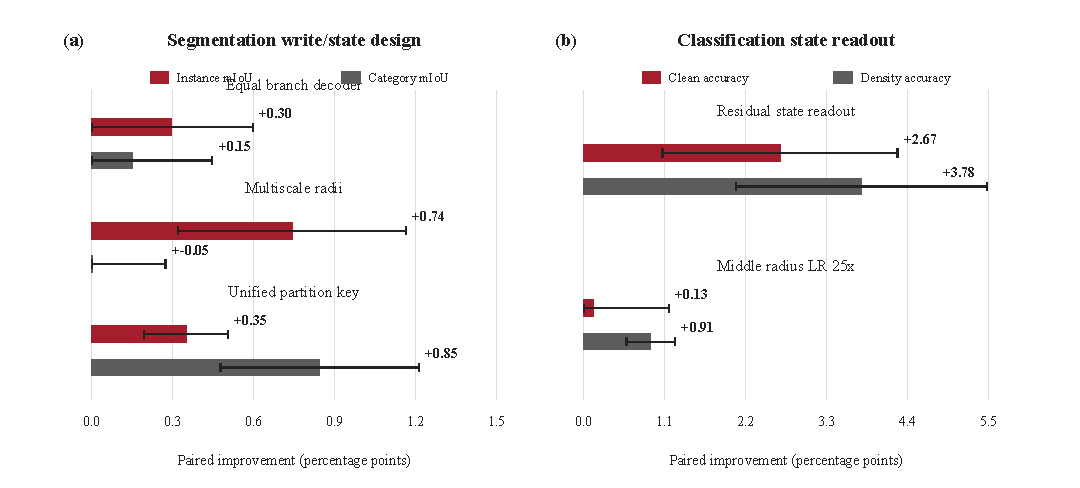
\includegraphics[width=0.92\linewidth]{fig03_controlled_ablation.pdf}
\caption{三种子、5 个 epoch 的架构筛选。柱表示配对均值变化，误差棒表示总体标准差。分割部分检验等宽分支解码器、不同半径初始化，以及统一的归一化空间地址；分类部分检验残差式与拼接式分支摘要，以及中尺度半径学习率。}
\label{fig:architecture-ablation-cn}
\end{figure}
这些筛选每次只隔离一个架构决策。所有筛选在同一比较内使用相同的数据划分与优化协议、5 个 epoch、种子 0/1/2，以及 2,048 个训练形状与 512 个测试形状的子集。这些短程运行用于选择结构性方案；正文主表报告的是在完整划分上 20 个 epoch 的最终结果。表~\ref{tab:screens-cn} 报告保留方案相对于所列替代方案的配对变化。

\begin{table}[t]
\centering
\caption{5 个 epoch 的受控筛选。正值表示支持保留方案。}
\label{tab:screens-cn}
\small
\begin{tabular}{p{0.27\linewidth}p{0.25\linewidth}p{0.36\linewidth}}
\toprule
保留的方案 & 配对的替代方案 & 配对变化\\
\midrule
分割：等宽解码器 & 中尺度解码器不等宽 & 实例 $+0.30\pm0.30$；类别 $+0.15\pm0.29$\\
分割：不同半径初值 & 相同半径初值 & 实例 $+0.74\pm0.42$；类别 $-0.05\pm0.33$\\
分割：统一归一化键 & 混合键定义 & 实例 $+0.35\pm0.16$；类别 $+0.85\pm0.37$\\
分类：中尺度残差 & 直接拼接 & 干净 $+2.67\pm1.60$；偏移 $+3.78\pm1.71$\\
分类：中尺度半径 $25\times$ 学习率 & 基础半径学习率 & 干净 $+0.13\pm1.03$；偏移 $+0.91\pm0.33$\\
\bottomrule
\end{tabular}
\end{table}

等宽的 $170\rightarrow160\rightarrow160$ 分割解码器使实例 mIoU 提升 $0.30\pm0.30$ 个百分点，并减少 24,480 个参数。不同的半径初始化使实例 mIoU 提升 $0.74\pm0.42$。对三个分支使用同一个归一化地址方程，相对混合键变体使实例与类别 mIoU 分别提升 $0.35\pm0.16$ 与 $0.85\pm0.37$。对纯状态分类，中尺度参考残差相对直接拼接使干净与密度偏移准确率分别提升 $2.67\pm1.60$ 与 $3.78\pm1.71$。只提高中尺度半径的学习率带来的干净准确率变化不稳定，但偏移准确率有稳定的 $0.91\pm0.33$ 提升；保留该设置正是为了这一稳定收益，而非其干净准确率效应。这些结果支持了所发布的读出头，同时使状态写入规则在三个分支间保持对称。

\section{讨论与局限}
本文设定的场景是不断增长或分布式的点流。传感器可以编码一帧、合并其状态，然后释放该帧。多台相机、激光雷达、机器人或边缘处理器可以在本地编码不相交的空间区域或时间窗，并把固定状态发送到服务器。相加随后得到与集中式编码相同的表示，因此聚合可以是异步且层次化的。原始点集无需离开感知设备。分割服务可以只保留它计划查询的坐标，而分类器在更新证据时无需重放更早的点。上述任何操作都不会把新点与此前解码过的所有点作比较。

\subsection{分布式推理示例}
设想若干激光雷达节点观测一个场景的不同部分。训练好的编码器被复制到每个节点，所有节点在同一参考系中以相同的归一化表达坐标。节点 $d$ 把它的本地分块编码为 $\{\Sstate_f^{(d)},\Sstate_m^{(d)},\Sstate_b^{(d)}\}$，随后即可删除本地特征。中继可以对这些三元组的任意子集求和；服务器再把中继的输出相加，得到式~\eqref{eq:distributed-cn}。到达顺序与通信树的形状都不影响实数运算下的结果。无论本地分块包含数百个点还是代表一段长的累计流，每个被传输的三元组都是同样的 255 KiB。

对分类，服务器把合并后的三元组直接送入状态行读出。新增一台设备或一帧只是再加一个三元组来改变类别证据，无需重新解码并池化更早的点云。对分割，服务器把坐标 $\bm q$ 送入三次矩阵读取。查询可以是选定观测点的坐标、操作员指定的区域，或规则网格上的位置；读取时只需要这些坐标可用。由于式~\eqref{eq:effective-read-cn} 对 $\bm q$ 光滑依赖，相邻查询会得到平滑变化的状态证据，包括在未被显式观测的坐标处。当前实验只在观测到的 ShapeNetPart 点上评估标签，因此在新坐标上的精度仍是一个开放的经验问题。

\subsection{表示的限制在哪里}
\label{sec:bottleneck-cn}
固定状态是摘要，而不是被压缩的点档案。它们足以求值所学到的读出头，但并不是为重建每一个原始观测而设计的。两个点集可能产生相近的矩表，尤其当许多空间地址相互重叠时。学习到的中心、半径、内容网络与二阶项决定了哪些区分能在这种压缩中存活。这既解释了有界内存的收益，也解释了与“保留或重建详细点关系”的邻域方法之间仍存在的精度差距。

更确切地说，一个点一旦被写入，状态就是之后任何阶段唯一能看到的东西，因此没有任何解码器能够恢复写入时已经丢弃的区分。所以，\textbf{状态而不是读出，才是该架构真正起约束作用的压缩瓶颈}。筛选实验直接支持这一点：改变分割解码器只使实例 mIoU 变化 $0.30\pm0.30$ 个百分点，改变其宽度或共享方式也只产生同量级的亚个百分点变化；而第~\ref{sec:parallel-cn} 节中改变状态配置则使其变化超过一个百分点。这正是本设计把结构预算花在“点如何被写入”——归一化地址、二阶值以及采用若干并行状态——而不是花在“状态如何被解码”上的原因，也解释了为什么加宽主状态无法替代并行结构。

PointNet++ 在观测点周围构建邻域，PointNet 保留逐通道极值，而 PointProgrammerNet 保留有限的矩表。对短点云而言状态开销还超过裸 XYZ 存储；其收益出现在有界通信、合并或长流足以抵偿这一固定成本的场景。分布式等价性要求完全相同的预处理与共享坐标系，分割仍需为每个被请求的坐标读取一次状态。评估仅限于 XYZ 输入、每个任务一个数据集、一块计时 GPU 与本地受控基线。未观测坐标上的精度、时序校准、更多属性以及 delta 自适应仍是未来工作。

\section{结论}
PointProgrammerNet 用固定的可加矩阵对点云作摘要。连续的键与二阶值支持无序写入、精确的分布式合并、移除、衰减，以及代价与历史长度无关的更新。若干并行状态所编码的可用结构多于同等参数预算下的单一状态，而真正起约束作用的压缩瓶颈是状态本身而非读出。坐标条件化的分割与纯状态的分类都在不对解码点做池化的情况下工作。精度仍低于层次化基线，但该模型为“从有界流式状态出发的集中式或分布式点云推理”提供了一个紧凑且可检验的设计。

\section*{声明}
\noindent\textbf{利益冲突。}作者声明不存在与本工作相关的经济或非经济利益冲突。

\noindent\textbf{资助。}本研究未接受任何资助。

\noindent\textbf{作者贡献。}Dian Yu：概念构思、方法学、软件、验证、形式分析、研究实施、数据管理、可视化、初稿撰写、审阅与编辑。

\noindent\textbf{数据可用性。}ShapeNetPart 与 ModelNet40 均为公开数据集，可从本文引用的原始来源获取。所发布的最小代码包含 341,909 参数的分割器与 529,426 参数的分类器、数据集加载器、训练循环、状态运算检查以及精确的三种子参考数值；\texttt{CODE\_REPRODUCTION.md} 说明了环境、数据集布局、命令与流式 API。可加性测试应在评估模式下运行，因为此时 BatchNorm 使用命题~\ref{prop:order-cn} 所假设的固定滑动统计量。

\bibliographystyle{unsrt}
\bibliography{references}
\end{document}
